\section{Servizio di Baking}
\label{sec:chapter_prove_sperimentali_servizio_baking}

In questo paragrafo verranno esposti i risultati riguardanti i test sulla velocità del servizio di baking, date in input delle scene 3D.
\\ 
La velocità del servizio è influenzata principalmente da due fattori:
\begin{itemize}
\item Il numero di oggetti all’interno della scena.
\item Il valore di sampling, che controlla qualità estetica del risultato;
\end{itemize}
Sono state quindi realizzate due differenti tipologie di test volte a misurare il tempo di processamento del baking delle lightmap, a fronte della variazione di questi due fattori.  

\subsection{Velocità al variare del numero di oggetti}
\label{sec:chapter_prove_sperimentali_servizio_baking_vel_obj}

Questa tipologia di test ha come obiettivo quello di sottomettere al servizio delle richieste di bake con scene di dimensione crescente, e per ogni richiesta misurare il tempo impiegato per elaborarla. 
\\
Il fattore variabile in questo test è la dimensione, quindi il numero di oggetti all’interno della scena. Altri fattori come l’illuminazione, che non inficia sensibilmente sulle performance, o il sampling, rimangono statici. 
\\
Il servizio permette di misurare il tempo effettivo di bake direttamente sul server, iniziando la misurazione esattamente al momento dell’istanziazione del processo di bake, e terminandola a fine processo. Pertanto le misure possono considerarsi fedeli, e non influenzate da fattori come i ritardi dovuti al traffico di rete. 
\\
A questo punto verranno mostrate le misure di velocità del servizio a fronte di cinque richieste di bake; ad ogni richiesta è associata una scena 3D contenente un numero di oggetti sparsi che va da 1 a 150. L’oggetto scelto in esame è un modello 3D di uso comune nell’arredamento di interni. 
\\
Per quanto riguarda l’illuminazione si è scelto di posizionare un’unica SpotLight all’interno della scena, mentre per il sampling è stato individuato un valore corrispondente ad un livello qualitivo medio-basso della scena in output, ossia 50. 
\\
Ogni richiesta è elaborata sfruttando due architetture hardware differenti: CPU e CUDA.
\\
I tempi di elaborazione delle richieste sono mostrati in tabella \ref{table:per_num_ob}:

\begin{table}[]
\centering
\caption[Performance al variare degli oggetti]{Tempi di bake, espressi in secondi, al variare del numero di oggetti.}
\begin{tabular}{|l|l|l}
\hline
\textbf{N. oggetti} & \textbf{Tempo di bake (CPU)} & \multicolumn{1}{l|}{\textbf{Tempo di bake (CUDA)}} \\ \hline
1 & 17.633 & \multicolumn{1}{l|}{8.871} \\ \hline
10 & 212.713 & \multicolumn{1}{l|}{91.86} \\ \hline
50 & 1640.517 & \multicolumn{1}{l|}{620.645} \\ \hline
100 & 3818.735 & \multicolumn{1}{l|}{1504.505} \\ \hline
150 & 4507.794 & \multicolumn{1}{l|}{1865.828} \\ \hline
170 & 5446.104 &  \\ \cline{1-2}
\end{tabular}
\label{table:per_num_ob}
\end{table}

Dalle misurazioni effettuate è possibile constatare come il numero di oggetti all’interno di una scena influenzi sensibilmente il tempo di bake. 
\\
Nonostate la scena sia composta da uno stesso oggetto ripetuto più volte, il tempo di bake incrementa in maniera non lineare con il numero di oggetti.
\\ 
Questo perchè incrementare il numero di oggetti all’interno della scena non solo ne aumenta la dimensione, ma comporta anche un carico computazionale maggiore per il Path Tracer di Blender, che dovrà calcolare un numero maggiore di rimbalzi dei raggi luminosi tra le superfici della scena.
\\
Spostando l’elaborazione del baking su architettura CUDA si nota immediatamente come le performance subiscano un incremento considerevole, con miglioramenti che in alcuni casi superano il 60\%, rispetto alle elaborazioni basate su CPU. 
\\
In figura \ref{fig:grafico1} e \ref{fig:grafico2} è possibile osservare come le performance aumentino considerevolmente utilizzando una architettura CUDA piuttosto che CPU.
\\
\begin{figure}[htb]
 \centering
 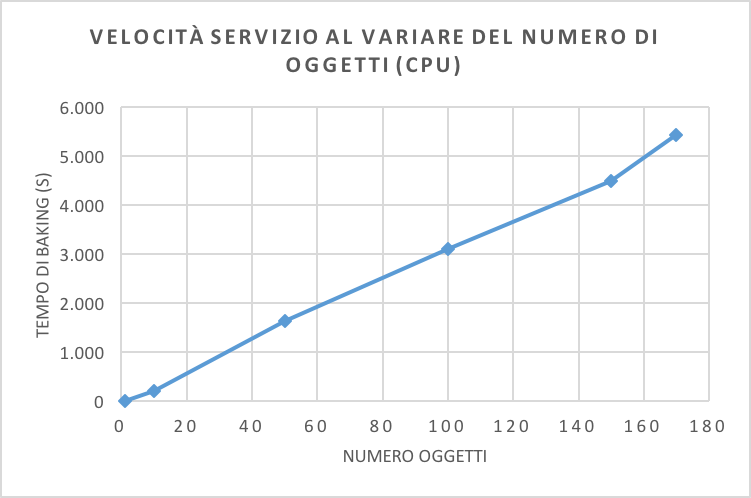
\includegraphics[width=0.8\linewidth]{images/chapter_prove_sperimentali/grafico1.png}\hfill
 \caption[Performance CPU variando oggetti]{Performance su architettura CPU del servizio di baking al variare del numero di oggetti.}
 \label{fig:grafico1}
\end{figure}
\\
\begin{figure}[htb]
 \centering
 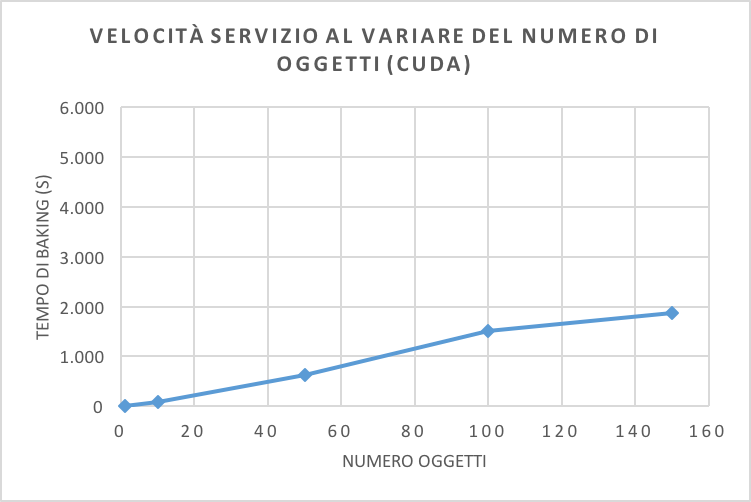
\includegraphics[width=0.8\linewidth]{images/chapter_prove_sperimentali/grafico2.png}\hfill
 \caption[Performance CUDA variando oggetti]{Performance su architettura CUDA del servizio di baking al variare del numero di oggetti.}
 \label{fig:grafico2}
\end{figure}

\subsection{Velocità e qualità al variare del sampling}
\label{sec:chapter_prove_sperimentali_servizio_baking_vel_sam}

Questa tipologia di test ha come obiettivo quello di sottomettere al servizio delle richieste di bake con scene di dimensione fissa, ma sampling variabile. 
\\
Il sampling è il parametro più importante per il controllo della qualità di un bake su di una scena 3D; per determinarne il valore è necessario raggiungere dei compromessi tra qualità desiderata e tempo che si è disposti ad attendere prima di ottenere il risultato. 
\\
Il range di valori di sampling scelto per i test corrisponde al processamento di  bake valoci ma di bassa qualità, fino al processamento di bake molto lenti ma di qualità elevata. Per la scena si è deciso di realizzare un ambiente di media complessità che contenesse un buon numero di oggetti ed ombre. Come per le misurazioni descritte nel paragrafo \ref{sec:hapter_prove_sperimentali_servizio_baking_vel_obj} , anche per questa attività di test vengono considerati i tempi di baking su due architetture hardware differenti: CPU e CUDA.
I tempi di elaborazione delle richieste sono mostrati in tabella \ref{table:per_samp} :

\begin{table}[]
\centering
\caption[Performance al variare del sampling]{Tempi di bake, espressi in secondi, al variare del sampling.}
\begin{tabular}{|l|l|l|}
\hline
\textbf{Sampling} & \textbf{Tempo di bake (CPU)} & \textbf{Tempo di bake (CUDA)} \\ \hline
1 & 162.8 & 79.364 \\ \hline
10 & 669.664 & 231.214 \\ \hline
30 & 1253.308 & 584.592 \\ \hline
50 & 1749.307 & 940.127 \\ \hline
80 & 2726.777 & 1505.961 \\ \hline
100 & 3361.082 & 1891.723 \\ \hline
150 & 4944.672 & 2719.677 \\ \hline
200 & 6547.286 & 3610.537 \\ \hline
300 & 9795.735 & 5437.929 \\ \hline
\end{tabular}
\label{table:per_samp}
\end{table}

Osservando le misure di velocità di processamento su architettura CPU in tabella \ref{table:per_samp} è possibile notare come il tempo di processamento aumenti in modo quasi lineare con il valore di sampling.
\\
Si prenda come riferimento il tempo di bake nel primo caso, ossia con valore di sampling pari a 1:
Il caso con sampling uguale a 10 è 4 volte più lento, mentre quello da 30 lo è circa 7 volte; quindi con un aumento di 20 punti di sampling il tempo tra i due casi aumenta di circa 3 volte il tempo impiegato nel caso di riferimento. Osservando il test da 50 sampling, rispetto a quello da 30 sampling anche qui si può notare un’aumento del tempo di bake di circa 3 volte, a fronte di un incremento del valore di sampling sempre di 20 punti. Salendo ancora è possibile notare come nei casi da 50 sampling, 100, 150 e 200, l’incremento di tempo è sempre lineare, e aumenta di 10 volte ogni incremento del valore di sampling di 50 punti. E’ dunque possibile individuare una crescita quasi lineare del tempo di processamento all’aumentare del valore di sampling.
\\ 
Questo tipo di andamento consente di avere dei tempi di processamento del bake prevedibili; ad esempio, prima di sottomettere una richiesta di bake con sampling alto, l’utente potrebbe sottomette una richiesta per un bake di qualità più bassa, utile come preview dell’aspetto finale che avrà la scena. Dal tempo impiegato per generare questa preview l’utente è in grado di stimare il tempo che sarà necessario per soddisfare la richiesta di bake di qualità più alta. 
\\
Si osservino ora i tempi per il calcolo degli stessi risultati sfruttando l’architettura CUDA. E’ possibile notare come le performance di bake migliorino del 45\% circa; questo incremento della velocità di elaborazione non è trascurabile, e dimostra come il calcolo parallelo su GPU sia molto più performante del tradizionale calcolo su CPU. I miglioramenti di un elaborazione su architettura CUDA rispetto che su architettura CPU vengono mostrati in figura \ref{fig:grafico3} e \ref{fig:grafico4} .
\\
\begin{figure}[htb]
 \centering
 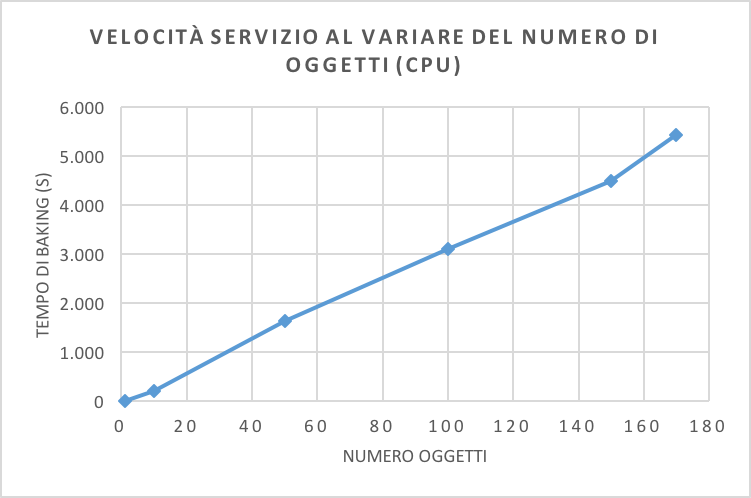
\includegraphics[width=0.8\linewidth]{images/chapter_prove_sperimentali/grafico1.png}\hfill
 \caption[Performance CPU variando sampling]{Performance su architettura CPU del servizio di baking al variare del sampling.}
 \label{fig:grafico3}
\end{figure}
\\
\begin{figure}[htb]
 \centering
 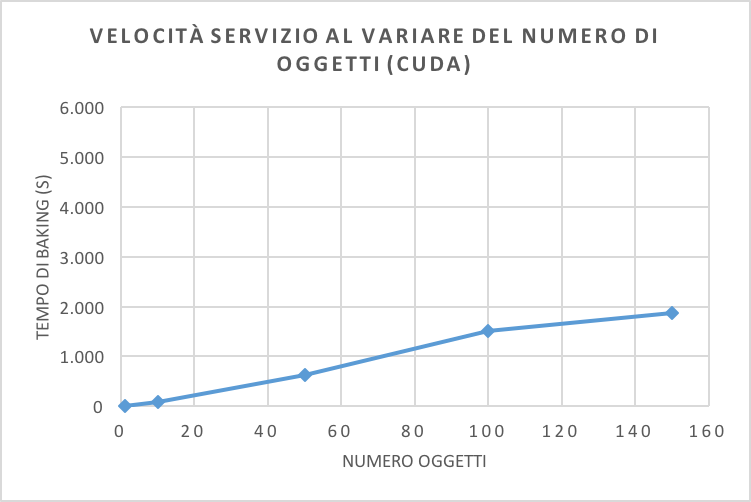
\includegraphics[width=0.8\linewidth]{images/chapter_prove_sperimentali/grafico2.png}\hfill
 \caption[Performance CUDA variando sampling]{Performance su architettura CUDA del servizio di baking al variare del sampling.}
 \label{fig:grafico4}
\end{figure} 

Come già menzionato il sampling è la caratteristica chiave per il controllo della qualità di un bake. Dopo aver mostrato come i tempi di processamento varino al variare del sampling, verrano ora mostrati gli output dei suddetti processamenti.
\\
Ogni output corrisponde ad una scena 3D su cui è stato effettuato un bake con un diverso livello di sampling; verranno mostrati i risultati per tre diversi valori di sampling, corrispondenti ad un livello qualitativo basso, medio e alto.
\\
Sarà possibile notare, per i tre diversi livelli di sampling, come il feedback visivo dal punto di vista della qualità cambi sensibilmente.
\\
\\
In figura \ref{fig:sampl1} viene mostrato il risultato di un baking delle lightmap con sampling a 1. Nonostante sia evidente la scarsa qualità dovuta all’aspetto estramamente sgranato degli effetti luminosi all’interno della scena, non è trascurabile il fatto che per generarla ci siano voluti poco meno di 3 minuti (circa 1 minuto con CUDA). 
\\
Da questo si può intuire che se si volesse generare una rapida anteprima di come sarà la scena, un bake con sapling a 1 è quantomeno in grado di fornire un’idea di come sarà l’illuminazione generale della scena, e della disposizione delle ombre all’interno della stessa.
\\
\begin{figure}[htb]
 \centering
 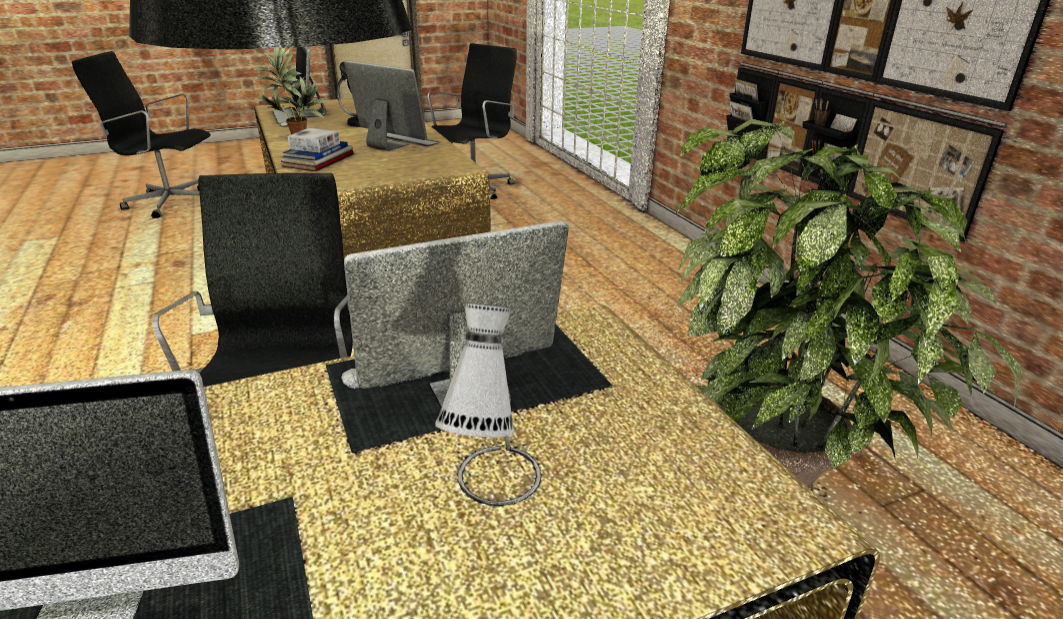
\includegraphics[width=0.8\linewidth]{images/chapter_prove_sperimentali/sampl1.png}\hfill
 \caption[Output sampling 1]{Output di un processo di bake con sampling uguale a 1.}
 \label{fig:sampl1}
\end{figure}

Per un livello qualitativo medio viene ora mostrato in figura \ref{fig:sampl50} il risultato di un bake con 50 sampling. 
\\
Come è possibile notare il livello di sgranatura degli effetti luminosi è calato sensibilmente, il che implica un’illuminazione generale molto più fedele e un’immagine decisamente più pulita.
\\
Nonostante ciò 50 è un valore di sampling non troppo alto, e nel risultato complessivo è ancora presente del rumore. Tuttavia la possibilità di ottenere tale risultato in circa 30 minuti (15 con CUDA) la rende una soluzione accettabile se si vuole giungere a compromessi con i tempi di servizio del sistema.
\\
\begin{figure}[htb]
 \centering
 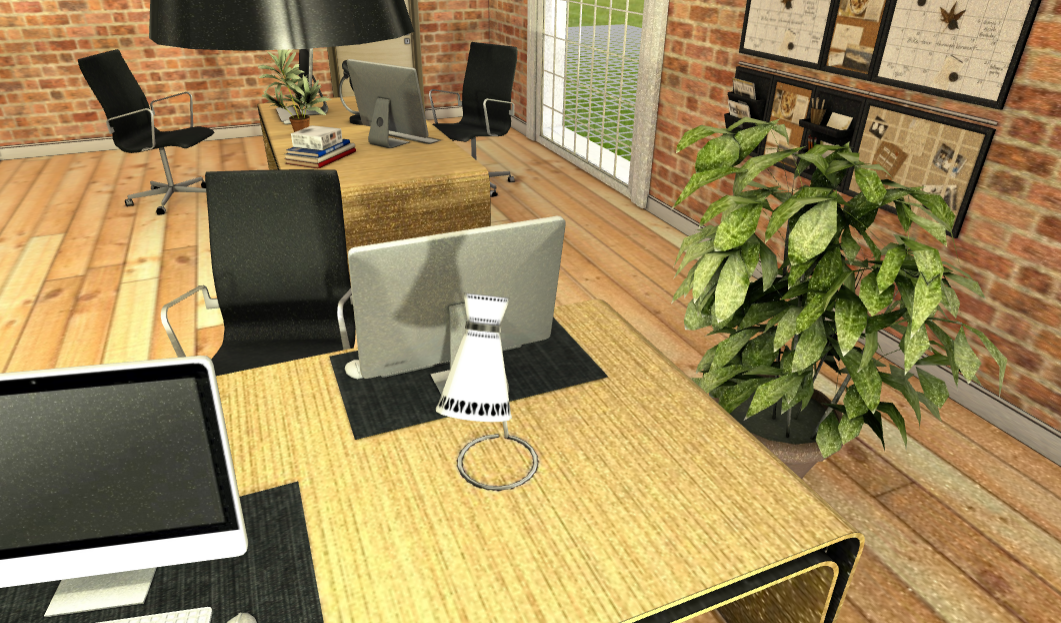
\includegraphics[width=0.8\linewidth]{images/chapter_prove_sperimentali/sampl50.png}\hfill
 \caption[Output sampling 50]{Output di un processo di bake con sampling uguale a 50.}
 \label{fig:sampl50}
\end{figure}

In conclusione è possibile notare in figura \ref{fig:sampl300} il risultato del baking con sampling più alto, ossia 300. Il rumore viene quasi completamente attenutato, ottenendo così un ottimo livello qualitativo della scena, a pattò però di attendere un tempo di processamento decisamente più lungo, di circa le 3 ore (1h30m con CUDA).
\\
\begin{figure}[htb]
 \centering
 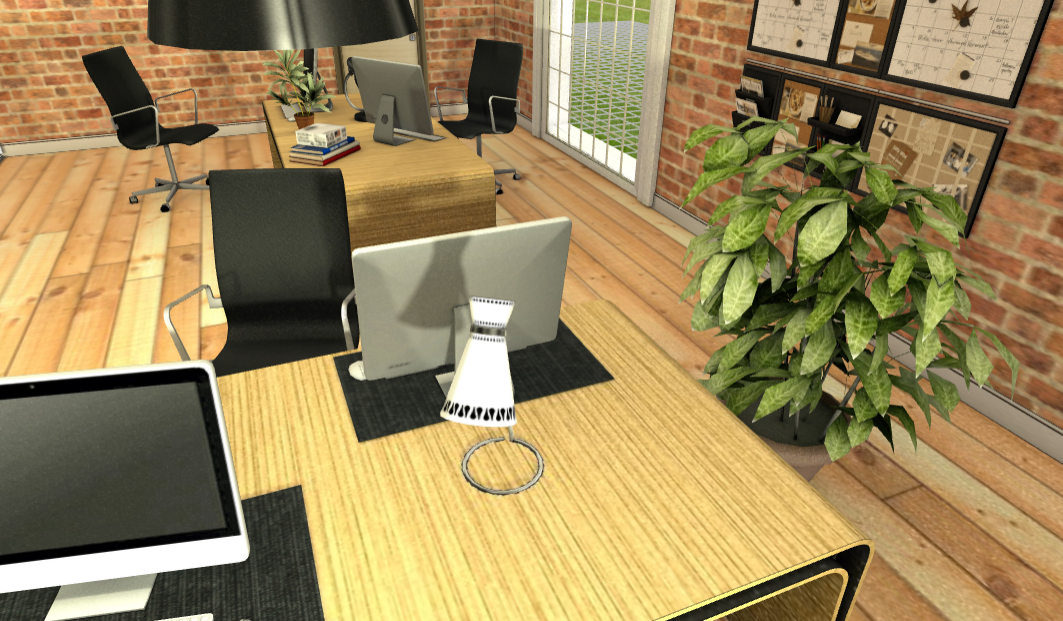
\includegraphics[width=0.8\linewidth]{images/chapter_prove_sperimentali/sampl300.png}\hfill
 \caption[Output sampling 300]{Output di un processo di bake con sampling uguale a 300.}
 \label{fig:sampl300}
\end{figure}

\subsection{Velocità al variare del numero di luci}
\label{sec:chapter_prove_sperimentali_servizio_baking_vel_luci}

Nei paragrafi precedenti sono state mostrate le attività di test volte a stressare il sistema intervenendo sui fattori che ne alterano sensibilmente le performance. Tra questi fattori sono state escluse le luci, e in questo paragrafo verrà mostrato come effettivamente il loro numero non inficia sul tempo di processamento del baking.
\\
Per testare se quanto affermato è effettivamente vero è stata realizzata un’attività di test in cui il servizio viene sottoposto a diverse richieste di bake, ognuna delle quali prevede una scena di input di dimensioni fisse e un numero di sorgenti luminose variabile. 
\\
La scena è composta da 30 oggetti di comune utilizzo nell’arredamento di interni, posizionati in punti casuali dello spazio. Le posizioni sono tutte contenute in un range tale da far si che ogni oggetto della scena possa essere irradiato da tutte le fonti luminose. 
\\
Tali fonti  luminose sono SpotLight con angolo e intensità di irradiazione costante. Per le attività di test sono state sottomesse 6 richieste differenti, con un numero di sorgenti luminose che varia da 1 a 20.
\\
Il sampling con cui viene richiesto il bake è costante e pari 50. 
Per ogni richiesta di bake è stato misurato il tempo di processamento; tutte le misure sono mostrate in tabella \ref{table:per_luci} .

\begin{table}[]
\centering
\caption[Performance al variare delle luci]{Tempi di bake, espressi in secondi, al variare del numero di luci all'interno della scena.}
\begin{tabular}{|l|l|}
\hline
\textbf{Numero luci} & \textbf{Tempo di elaborazione (CPU)} \\ \hline
1 & 656.002 \\ \hline
4 & 653.477 \\ \hline
7 & 657.825 \\ \hline
10 & 650.662 \\ \hline
15 & 662.986 \\ \hline
20 & 661.54 \\ \hline
\end{tabular}
\label{table:per_luci}
\end{table}

Come è possibile notare dai risultati in tabella \ref{table:per_luci} , il tempo processamento di bake rimane pressochè costante indipendentemente dal numero di luci aggiunte. 
\\
Questa particolarità è del tutto motivata dall’algoritmo di illuminazione indiretta utilizzato dal motore di render scelto in Blender per eseguire il baking. 
\\
Come già visto nel paragrafo \ref{sec:chapter_tecnologie_abilitanti_blender} il motore di render scelto è un Path Tracer, che prende il nome dall’omonimo algoritmo di illuminazione utilizzato; tale algoritmo si basa sulla caratterista di lanciare dei raggi dalla camera attraverso ognuno dei pixel nel piano di immagine descritto dalla camera stessa; ogni raggio può o meno colpire una fonte luminosa presente nella scena, determinando quindi se il pixel del piano di immagine da cui il raggio è emesso deve essere illuminato o meno. 
\\
Siccome i raggi vengono emessi dalla camera, e non dalle fonti luminose, il loro numero è totalmente indipendente dalla quantità di luci presenti nella scena. 
\\
Inoltre se considerato che per ogni scena il numero degli oggetti e la loro posizione rimane invariata, le collisioni parzialmente randomiche dei raggi con le superfici della scena rimangono pressochè invariate.
\\ 
Questa caratteristica dell’algoritmo di illuminazione fa si che i tempi di processamento mostrati in tabella \ref{table:per_luci} oscillino intorno ad un valore costante; questa condizione permette all’utente di arricchire la scena costruita nell’Editor con un numero di fonti luminose anche elevato, a patto che l’hardware a disposizione riesca a sostenere la crescente mole di carico computazionale. Nel capitolo \ref{sec:chapter_prove_sperimentali_navigator} verrà mostrato come la quantità di luci all’interno della scena, pur non inficiando le performance del servizio di bake, può influire negativamente sulla fruibilità della scena all’interno dell’editor o del navigator.

\subsection{Dimensione del JSON output al variare del numero di oggetti}
\label{sec:chapter_prove_sperimentali_servizio_baking_dim_obj}

Le attività di test mostrate fino a questo punto hanno avuto come scopo unico quello di misurare la velocita del servizio di bake, intesa come quantità di tempo impiegata per elaborare la richiesta di bake sottomessa dall’utente. 
\\
Questo paragrafo vuole concentrare l’attenzione su un’altro aspetto fondamentale, ossia la dimensione dei risultati prodotti dal servizio di bake; nel pragrafo \ref{sec:chapter_architettura_sistema_formato_scambio} è stato già mostrato come la scena costruita dall’utente nell’editor venga memorizzata in un file JSON, in cui vige un formato di intercambio dei dati fruibile dall’Editor così come dal Servizio di baking e dal navigator.
\\
In una tipica attività di costruizione di una scena 3D, è possibile che l’utente decida di memorizzare la scena in più fasi del processo costruttivo, ottenendo quindi un numero variabile di file JSON che devono essere memorizzati su disco. Pertanto il JSON deve necessariamente avere dimensioni contenute, il che per giunta ne semplifica l’eventuale interscambio con altri utenti. 
\\
Altro vantaggio non trascurabile è il fatto di avere un volume di dati ridotto da dover inviare al servizio di bake: come già discusso nel paragrafo \ref{sec:chapter_baking_service_architettura_servizio} le richieste di bake vengono sottomesse ad un servizio in remoto, pertanto le informazioni sulla scena sono trasferite via internet. Tali informazioni devono avere un volume contenuto, al fine di non appesantire troppo il traffico di dati, e garantire un tempo di ricezione della richiesta accettabile. 
\\
Gli interventi sull’ottimizzazione delle dimensioni del file JSON rappresentante la scena, sono per lo più mirate a ridurre la dimensione dei data URL delle immagini utilizzate per texturizzare le superfici dei modelli.
\\
Inoltre nel paragrafo \ref{sec:chapter_lrl_li_te_ba} è stato mostrato come il processo di Blender si impegni nella generazione di nuove immagini chiamate Lightmapped Textures, che andranno a sostituire nella descrizione della scena le immagini preesistenti.
\\
Siccome i data URL delle immagini sono il dato più pesante all’interno di un file JSON, qualsiasi attività di ottimizzazione effettuata sulle immagini lato client dovrà essere ripetuta sulle lightmapped texture prima di inviare il risultato; tale mansione viene presa in carico direttamente dal processo di Blender.
\\
Ciò che verrà mostrato in questo paragrafo sono i risultati di due differenti attività di test, volte a mostrare la capacità di compressione dei risultati da parte del servizio. 
\\
Nella prima attività di test verrano sottomesse al servizio delle richieste contenenti scene con un numero crescente di oggetti; al termine del processamento verrà estratta la dimensione dell’output e la si compara con quella della scena inviata nella richiesta. 
\\
Le scene utilizzate per questo test sono composte da oggetti di uso comune nell’arredamento di interni. 
\\
Illuminazione e sampling sono fissati, e il numero di oggetti varia da 1 fino ad un massimo di 150 oggetti. In tabella \ref{table:dim_obj} vengono mostrate le dimensioni dei file JSON prodotti nell'editor, e le dimensioni degli stessi file JSON elaborati mediante servizio di bake.

\begin{table}[]
\centering
\caption[Confronto dimensioni input-output]{Confronto tra dimensione del JSON input prodotto dal servizio editor, e dimensione del JSON output prodotto dal servizio di bake.}
\begin{tabular}{|l|l|l|}
\hline
\textbf{Numero oggetti} & \textbf{Dimension input (Mb)} & \textbf{Dimensione output (Mb)} \\ \hline
1 & 1.4 & 0.2526 \\ \hline
10 & 14.3 & 2.4 \\ \hline
50 & 71.6 & 11 \\ \hline
100 & 143.3 & 21.2 \\ \hline
150 & 214.9 & 33.5 \\ \hline
\end{tabular}
\label{table:dim_obj}
\end{table}

Come è possibile notare in tabella \ref{table:dim_obj} , le dimensione degli output del processo di bake corrispondono a circa il 16\% dei rispettivi input, segno di un ottimo fattore di compressione. Il grafico in figura \ref{fig:grafico5} mostra come la dimensione dei JSON prodotti dal servizio di bake rimanga contenuta anche per input di dimensioni notevoli.
\\
\begin{figure}[htb]
 \centering
 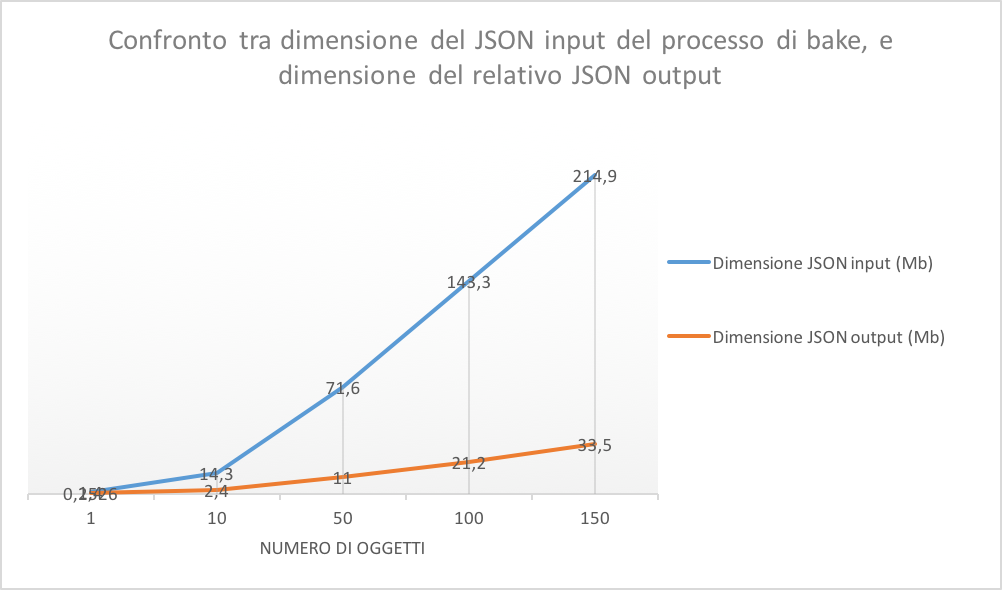
\includegraphics[width=0.8\linewidth]{images/chapter_prove_sperimentali/grafico5.png}\hfill
 \caption[Confronto dimensioni input-output]{Dimensioni del JSON input e JSON output messe a confronto per scene con numero di oggetti variabile.}
 \label{fig:grafico5}
\end{figure}

Grazie a ciò è possibile fruire di scene anche molto complesse, con un consumo di memoria su disco decisamente ridotto. 
\\
Un’esempio pratico è la riproduzione dell’ambiente domestico mostrato nel paragrafo \ref{sec:chapter_prove_sperimentali_qualita_visiva}. Nonostante la costruzione abbia portato ad una scena dalle dimensioni corpose, circa 117 Mb, è stato possibile ottenere una versione fotorealistica della stessa con 54.2 Mb. Trattandosi di un’intera abitazione il risultato può considerarsi soddisfacente.
\\
Si consideri che la compressione effettuata del processo di Blender è il giusto compromesso tra qualità e spazio occupato in memoria; è in verità possibile aumentare ulteriormente il fattore compressione, tuttavia dalle numerose sperimentazioni svolte la configurazione attuale può ritenersi ottimale.
\\
\\
La seconda attività test pone ancora l’attenzione sulla capacità di compressione dei dati da parte del servizio di baking, ma relazionando la dimensione dell’output al fattore di sampling del processo di bake. 
\\
Tale test vuole infatti mostrare come la riduzione del rumore a seguito di un bake con sampling più alto, migliori notevolmente la capacità di compressione dei risultati da parte del sistema.
\\ 
Questa attività prevede dunque la sottomissione al servizio di una serie di richieste di bake, aventi scena immutata ma sampling variabile. 
\\
Per la scena si è scelto di utilizzare lo stesso ambiente oggetto dei test descritti nel paragrafo \ref{sec:chapter_prove_sperimentali_servizio_baking_vel_sam}. 
\\
Ad ogni richiesta corrisponde un bake di qualità differente, che va dalla qualità più bassa (sampling = 1), ad un livello qualitivo molto alto (sampling = 300). Nella tabella \ref{table:dim_sam} sono mostrate le dimensioni dell’output in corrispondenza di ogni valore di sampling.

\begin{table}[]
\centering
\caption[Dimensioni output variando sampling]{Dimensione del JSON output al variare del sampling.}
\begin{tabular}{|l|l|}
\hline
\textbf{Sampling} & \textbf{Dimensione output} \\ \hline
1 & 39.2 \\ \hline
10 & 33.7 \\ \hline
30 & 32.3 \\ \hline
50 & 31.5 \\ \hline
80 & 30.4 \\ \hline
100 & 30 \\ \hline
150 & 29.2 \\ \hline
200 & 28.8 \\ \hline
300 & 28.1 \\ \hline
\end{tabular}
\label{table:dim_sam}
\end{table}

Come è possibile notare in tabella \ref{table:dim_sam} , mentre con un sampling uguale a 1 si ottiene un’output che in dimensione è il 90\% dell’input, con un fattore di sampling uguale a 300 si riesce ad ottenere una dimensione dell’output pari a circa il 64\% di quella del rispettivo input. 
\\
La motivazione principale a favore di questo miglioramento è il fatto che ad elevati valori di sampling le immagini realizzate dal processo di baking sono molto meno rumorose, pertanto la compressione risulta più efficace. 
\\
Ne è prova ulteriore la comparazione mostrata in figura \ref{fig:dim_sam} , dove vengono messe a contronto due lightmapped texture generate a partire da uno stesso input: la prima texture è prodotta mediante processo di bake con sampling pari a 1, mentre 50 è il valore di sampling del bake che ha generato la seconda.
\\
\begin{figure}[htb]
 \centering
 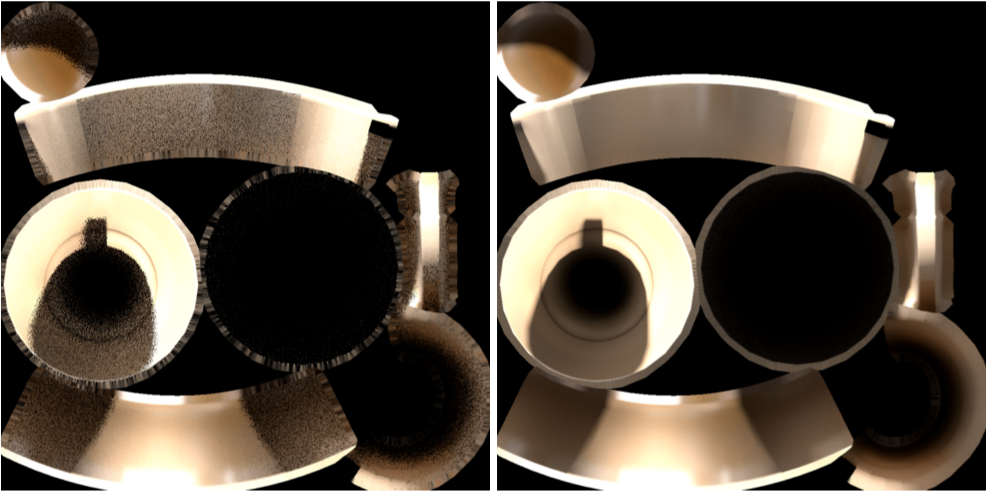
\includegraphics[width=1\linewidth]{images/chapter_prove_sperimentali/dim_sam.png}\hfill
 \caption[Confronto dimensione lightmapped texture]{Una lightmapped texture realizzata con sampling uguale a 1 (a sinistra), e 50 (a destra)}
 \label{fig:dim_sam}
\end{figure}

Come è possibile notare in figura \ref{fig:dim_sam} la prima immagine presenta del rumore significativo, mentre la seconda è decisamente più pulita.
\\ 
Il particolare fondamentale che distingue le due foto, oltre all’aspetto qualitativo, è la dimensione: mentre la prima immagine pesa 1.3 Mb, la seconda ha una dimensione di 1 Mb, e questo con un sampling pari a 50. 
\\
Dalle misurazione mostrate in tabella \ref{table:dim_sam} si può facilmente dedurre che la dimensione possa diminuire ulteriormente per valori di sampling più alti.